\chapter{Aufgabe 1}

\section{a)}
\textit{Skizzieren Sie den internen Aufbau einer kontaktbehafteten Chipkarte und charakterisieren Sie die einzelnen Komponenten.}\\

\noindent
Die Skizze einer kontaktbehafteten Chipkarte ist in Abbildung~\ref{fig:chipkarte} angegeben.
Es erfolgt eine allgemeine Beschreibung von Chipkarten und der darin verwendeten Komponenten:

\begin{itemize}
    \itemsep0.5em
    \item Chipkarten gibt es in unterschiedlichen Bauformen, die über ISO 7810 standardisiert sind.
    Die Chips selber sind in einen Kartenkörper eingefasst, der meist aus PVC (\textit{Polyvinylchlorid}) besteht.
    \textit{Schartner} stellt einige der o.a. Bauformen in~\cite[]{ITS5} vor, darunter \textit{ID-1}, \textit{ID-00}, \textit{ID-000}, \textit{Mini-UICC}, wobei dem Format und dem Einsatzzweck der Chipkarte nach weitere \textit{optische} Informationen auf der Karte selber untergebracht werden können, die bspw. zur Personalisierung der Karte und Identifikation des Kartenbesitzers dienen, darunter u.a. Namen/ID-Nummern (Bank-/Kreditkarte), \textit{Profilfoto} des Besitzers, schwer zu fälschende Muster und Zeichen (\textit{Hologramme}, \textit{Guillochen}, vgl.~\cite[74]{ITS5}).\\
    Erwähnenswert sind in diesem Zusammenhang \textit{Hybridkarten}, die neben einem Chip auch noch einen Magnetstreifen besitzen, um eine gewisse Kompatibilität zu anderen Lesegeräten herzustellen (\cite[4]{ITS5}).

    \item Der in den Kartenkörper eingefasste Chip besitzt unterschiedliche Segmente, die bestimmte Funktionalitäten realisieren.
    Diese werden im Folgenden kurz beschrieben:
    \begin{itemize}
        \item Ohne auf Details einzugehen, lässt sich die Architektur des Chips wie folgt beschreiben: Die CPU des Chips ist über einen Bus mit den verschiedenen \textit{Speichereinheiten} verbunden. Chipkarten, die die Sicherheitsziele \textit{Integrität}, \textit{Authentizität} und \textit{Vertraulichkeit} umsetzen, verteilen die Daten auf Speicherbereiche, die ein \textit{Lesen}, \textit{Löschen}, \textit{Ändern} unterschiedlich kombiniert erlauben: So ist der \textit{(P)ROM} dafür verantwortlich, das Betriebssystem unveränderlich zu speichern, \textit{EEPROM} dient als nichtflüchtiger Speicher, der (Sitzungs-)Daten speichern und wieder zur Verfügung stellen kann, und der \textit{RAM} dient auch hier - wie aus anderen Rechnerarchitekturen bekannt - als (flüchtiger) Arbeitsspeicher.

        \item Damit die Karte überhaupt in den Betriebsmodus übergehen kann, muss der Chip (die CPU) mit Spannung versorgt werden. Hierzu dient das in der Abbildung angegebene Segment \textbf{C1}.

        \item Sobald die CPU mit Energie versorgt wird, kann ein Terminal über das Segment \textbf{C2} einen ``Reset`` der Karte veranlassen, woraufhin die Kommunikationssitzung von der Karte über ein sogenanntes \textit{ATR} (\textit{Answer to Reset}) bestätigt werden kann.

        \item Zur \textit{seriellen} Kommunikation dient das Segment \textbf{C7} (\textit{Input} / \textit{Output}), wobei die Synchronisation zwischen Terminal und Karte über das Segment \textbf{C3} (\textit{CLK} - Clock, Takt) realisiert wird.
    \end{itemize}
\end{itemize}

\begin{figure}
    \centering
    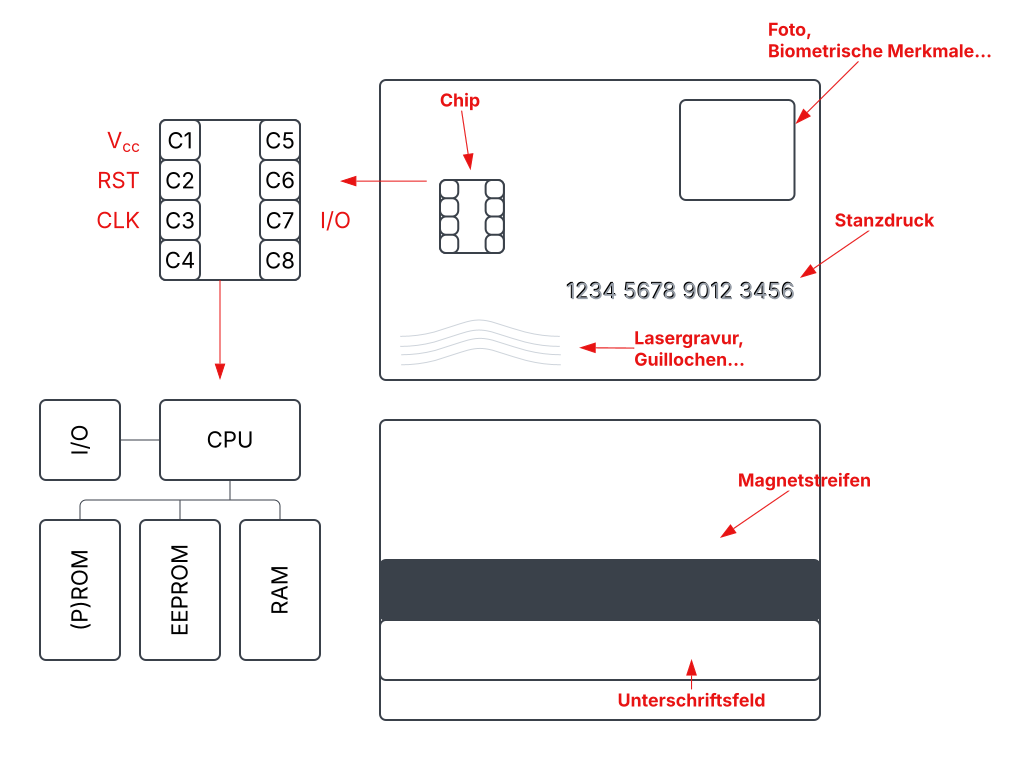
\includegraphics[scale=0.4]{aufgabe 1/img/chipkarte.svg}
    \caption{Skizzenhafte Darstellung einer kontaktbehafteten Chipkarte (Vorderseite oben, Rückseite unten) und möglicher Komponenten. (Quelle: in Anlehnung an~\cite[\textbf{Abb. 2.1}, 9 sowie \textbf{Abb. 2.2}, 10]{ITS5})}
    \label{fig:chipkarte}
\end{figure}


\section{b)}

\textit{Welche Komponenten werden für eine Dual‐Interface‐Chipkarte zusätzlich benötigt?}\\

\noindent
Als \textit{Dual-Interface-Chipkarten} (auch: \textit{Kombikarte},~\cite[4]{ITS5}) werden diejenigen Chipkarten bezeichnet, die sowohl \textit{kontaktlos} als auch \textit{kontaktbehaftet} mit einem Terminal kommunizieren können.\\
Da die Energieversorgung solcher Karten über \textit{elektromagnetische} oder \textit{kapazitive Kopplung} erfolgt, sind Schreib-/Lesedistanzen zwischen Terminal und Karte begrenzt (vgl.~\cite[27]{ITS5}).

\noindent
Damit bspw. kontaktlos nach ISO 14443\footnote{
    \url{https://en.wikipedia.org/wiki/ISO/IEC_14443}, abgerufen 15.04.2025
} kommuniziert werden kann, benötigt die Karte als \textit{physische Voraussetzung} eine Komponente zum Senden/Empfangen von Daten, was über ein in die Karte eingelassenes \textit{RFID}\footnote{
    \textit{Radio-Frequency Identification} (\cite[95 f.]{ITS5})
}-Modul/ eine \textit{RFID}-Antenne realisiert wird (vgl.~\cite[27]{ITS5}).

\noindent
\textit{Logisch} benötigt der Prozessor als zusätzliche Komponente ein Interface zur Verarbeitung und Umsetzung der Protokolle, die mit der Funktechnologie einhergehen, wie es bspw. der \textit{Infineon SLE 66CLX800PE}\footnote{
    s.a.~\url{https://www.electronicsdatasheets.com/manufacturers/infineon-technologies-ag/parts/sle-66clx800pe-ms}, abgerufen 15.04.2025
}  anbietet (vgl.~\cite[11]{ITS5}).

\section{c)}

\textit{Skizzieren und beschreiben Sie das Prinzip der Kommunikation zwischen einer
kontaktbehafteten Chipkarte und einem Terminal (einschließlich Kontaktierung
und Verbindungsaufbau).}\\

\noindent
Es erfolgt eine skizzenhafte Beschreibung der Kommunikation zwischen Terminal und Karte (kontaktbehaftet), wobei sich einige Beschreibungen auf die Darstellung in~\ref{fig:chipkarte} beziehen.\\

\noindent
\begin{enumerate}
    \item Sobald der Kontakt zwischen Karte und Terminal hergestellt ist, wird die Karte über \textbf{C1} mit Spannung und \textbf{C3} mit dem Takt versorgt.
    \item Das Terminal sendet \texttt{RESET} über \textbf{C2} und initiiert die Kommunikation, was umgangssprachlich einen ``Bootvorgang`` der Chipkarte auslöst (\textit{Power-on-Reset}, \cite[22]{ITS5}).
    \item Die Karte antwortet (standardisiert) mit einem \texttt{ATR} (\textit{Answer-To-Reset}), wobei die Karte dem Terminal weitere Informationen (unterstützte Kommunikationsprotokolle, Betriebssystem, \ldots) für die Sitzung bereitstellen kann.
    \item Die Kommunikation erfolgt nachfolgend im \textit{Leader-Follower}- bzw. \textit{Client-Server}-Modus\footnote{
    wir vermeiden an dieser Stelle absichtlich die im Skript notierte \textit{Master-Slave}-Terminologie unter Verweis auf die Diskussion in \url{https://en.wikipedia.org/wiki/Master-slave_(technology)}, Abschnitt \textit{Controversy} (abgerufen 15.04.2025)
    }: Das Terminal \textit{Leader} gibt die Befehle vor, die Karte (\textit{Follower}) reagiert entsprechend.
    \item Bei Entnahme der Karte bzw. durch einen Mechanismus der Terminals wird die Energieversorgung der Karte unterbrochen (und die Karte zur Entnahme angeboten).
    \item Der flüchtige Speicher verliert seine Informationen, ggf. in den \textit{EEPROM} eingetragene Daten bleiben erhalten.
    Sobald die Karte wieder in ein Terminal eingeführt wird: Starte mit Schritt 1.
\end{enumerate}


\section{d)}

\textit{Wofür steht die Abkürzung APDU?}\\

\noindent
Die Abkürzung \textit{APDU} steht für \textit{Application Protocol Data Unit} und bezeichnet ein Kommunikationspakete bzw. \textit{Nachrichten}, die bei der Kommunikation zwischen Karte und Terminal ausgetauscht werdeb.\\
Ein APDU kann dabei in Form eines \textit{Command-APDUs} von dem Terminal zu dem Betriebssystem der Karte auftreten, und entsprechend mit einem \textit{Response-APDU} von dem Betriebssystem (nach Abarbeitung auf Anwendungsschicht) beantwortet werden.
Der Ablauf ist skizzenhaft in Abbildung~\ref{fig:apdu} dargestellt.


\begin{figure}
    \centering
    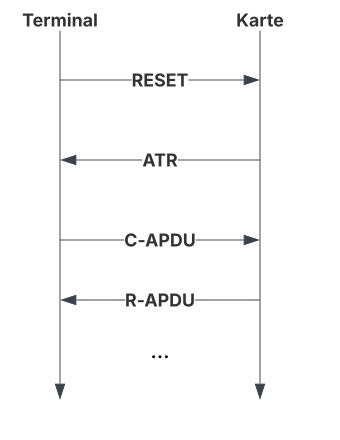
\includegraphics[scale=0.4]{aufgabe 1/img/apdu.svg}
    \caption{Skizzenhafte Darstellung der Kommunikation zwischen Termin und Karte. Nicht dargestellt ist hier die weitere Aushandlung von protokollspezifischen Parametern, \textit{PPS} (\textit{Protocol Parameter Selection}) genannt, was nach dem \texttt{ATR} geschehen kann. (Quelle: in Anlehnung an~\cite[\textbf{Bild 6.1}, 378]{RF02})}
    \label{fig:apdu}
\end{figure}


\section{e)}

\textit{Beschreiben Sie den Aufbau von Command‐ und Response‐APDUs und nennen
Sie jeweils ein Beispiel für die vier möglichen Kombinationen aus Command‐
und Response‐APDU (Case 1 bis Case 4).}\\


\noindent
Der Aufbau von Command- und Response-APDU ist jeweils in Abbildung~\ref{fig:capdu} und~\ref{fig:rapdu} dargestellt.\\
Es folgt eine kurze Beschreibung der einzelnen Felder der Nachrichtenpakete (vgl. i.F.~\cite[23 ff.]{ITS5} sowie~\cite[430 ff.]{RF02}).

\subsection*{Command APDU}

Eine Command APDU besteht aus folgenden Feldern (s. Abbildung~\ref{fig:capdu}):

\begin{itemize}
    \itemsep0.5em
    \item \texttt{CLA} (\textit{Class-Byte}): Kennzeichnet Anwendungen und ihren Befehlssatz (ISO-Anwendungen bspw. gekennzeichnet durch \code{0X}\footnote{
    In dieser Schreibweise entspricht $0$ dem msb, $X$ eine beliebige Anordnung niederwertiger Bits.
    }
    \item \texttt{INS} (\textit{Instruction-Byte}): Eigentlicher Befehl
    \item \texttt{P1}/ \texttt{P2}: \textit{Parameter-Bytes}, die \textt{INS} näher beschreiben
    \item \texttt{Lc} (\textit{Length Command}): Länge des gesendeten Datenfelds \texttt{cData}
    \item \texttt{cData}: Nutzdaten (kann leer sein)
    \item \texttt{Le} (\textit{Length expected}): Erwartete Länge des Datenteils der Response
 \end{itemize}

\begin{figure}
    \centering
    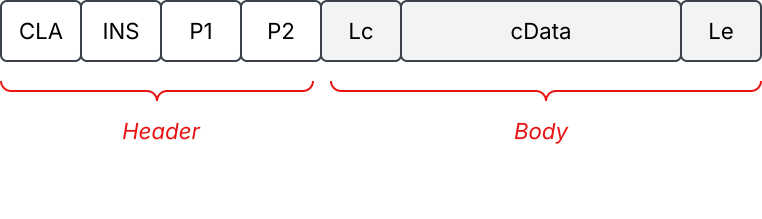
\includegraphics[scale=0.4]{aufgabe 1/img/capdu.svg}
    \caption{Struktur einer Command APDU. (Quelle: in Anlehnung an~\cite[\textbf{Abb 2.5}, 23]{ITS5})}
    \label{fig:capdu}
\end{figure}


\subsection*{Response APDU}

Da die Protokollarchitektur dem \textit{Leader-Follower-Prinzip} entspricht, gehen die Commands immer vom Terminal aus - jeder Command muss von der Karte über eine Response APDU beantwortet werden, weshalb eine Zuordnung \textit{Nachricht $\rightarrow$ Antwort} synchron erfolgt und keine weiteren Header-Informationen von dem Client aus benötigt wird, was sich in der schlanken Struktur von Response APDUs niederschlägt (s. Abbildung~\ref{fig:rapdu}):

\begin{itemize}
    \itemsep0.5em
    \item \texttt{rData}: Datenfeld
    \item \texttt{SW1}/ \texttt{SW2} (\textit{Return-Codes}, jeweils ein Byte): Enthalten Status-Codes bzgl. des empfangenen/abgearbeiteten Befehls (bspw. \code{0x9000} als Hinweis auf eine fehlerfreie Ausführung)
\end{itemize}

\begin{figure}
    \centering
    
\includegraphics[scale=0.4]{aufgabe 1/img/rapdu.svg}
    \caption{Struktur einer Response APDU. (Quelle: in Anlehnung an~\cite[\textbf{Abb 2.6}, 24]{ITS5})}
    \label{fig:rapdu}
\end{figure}


\subsection*{``Cases``}

Eine Command APDU besteht aus einem optionalen Datenteil, nämlich dem \textit{Body}.
Darüber hinaus muss nicht jeder Command auch eine Antwort erwarten - dadurch ergeben sich die in Abbildung~\ref{fig:cases} dargestellten Fälle bzgl. der Struktur einer Command APDU:

\begin{enumerate}
    \itemsep0.5em
    \item \textbf{Nur Header}: Übertragung von Protokollinformationen an die Karte, die nur mit einem Status antwortet.
    \item \textbf{Nur Header und Le-Feld}: Übertragung von Protokollinformationen.
    Karte antwortet mit Nutzlast in angegebener Länge und Statusinformationen (ggf. ohne Nutzlast, falls Fehler auftritt), bspw. wenn das Terminal die Karte sperrt.
    \item \textbf{Header, Lc- und Daten-Feld}: Übertragung von Nutzdaten an die Karte mit der angeg. Länge. Das Terminal erwartet keine Nutzlast in der Antwort. Die Karte antwortet mit den Statusbytes. Ein möglicher Anwendungsfall wäre hier das Speichern von in der Nutzlast enthaltenen Daten.
    \item \textbf{Header, Lc-, Le- und Daten-Feld}: Übertragung von Nutzdaten an die Karte. Das Terminal erwartet eine Antwort im Sinne einer ``vollwertigen`` Response APDU (Nutzdaten und Statusbytes). Ein möglicher Anwendungsfall ist die Erstellung einer Signatur basierend auf einem in der Karte gespeicherten privaten Schlüssels.
\end{enumerate}



\begin{figure}
    \centering
    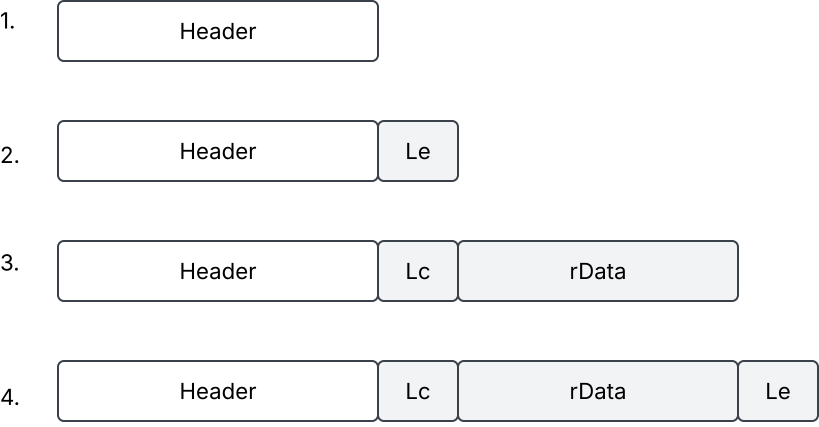
\includegraphics[scale=0.4]{aufgabe 1/img/cases.svg}
    \caption{Struktur einer Command APDU. (Quelle: in Anlehnung an~\cite[\textbf{Bild 6.41}, 431]{RF02})}
    \label{fig:cases}
\end{figure}
